\documentclass[14pt]{resume}
\usepackage{graphicx}
\usepackage{tabu}
\usepackage{multirow}
\usepackage{multicol}
\usepackage{progressbar}
\usepackage{linespacing_fix}
\usepackage{cite}

% Windows系统使用
%\usepackage{xeCJK}
%\setCJKmainfont{SimSun}

% Mac系统使用
\usepackage{xeCJK}
\setCJKmainfont[BoldFont=STHeiti,ItalicFont=STKaiti]{STSong}
\setCJKsansfont[BoldFont=STHeiti]{STXihei}
\setCJKmonofont{STFangsong}


\begin{document}
\pagenumbering{gobble}

\begin{multicols}{4}
    \Large{
        \begin{tabu}{ r }
            \multirow{5}{1in}{
                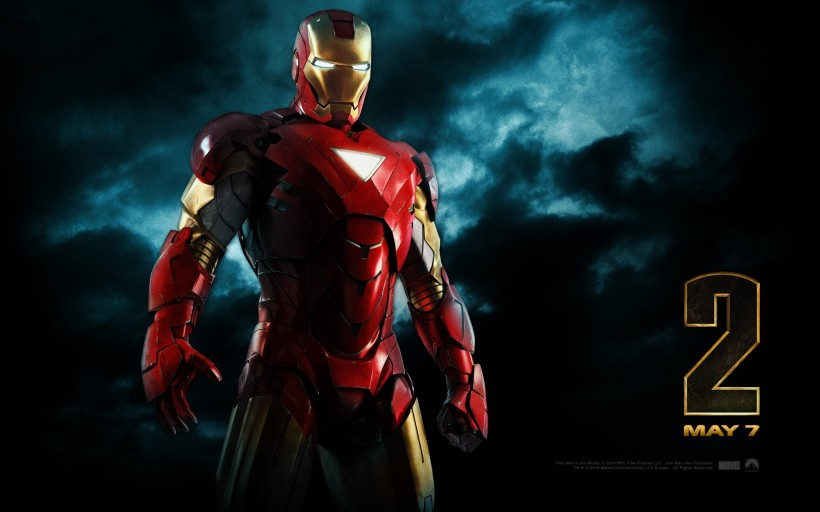
\includegraphics[width=0.88in]{avatar}
            }
        \end{tabu}
    }
    \columnbreak
    \Large{
        \begin{tabu}{ l l }
            & \faBirthdayCake{1993.01.01} \\
            & \phone{(+86)156-0000-0000} \\
            & \email{***@gmail.com} \\   %@qq.com
            & \github[github.com/***]{https://github.com/***} 
		\\
		\\
        \end{tabu}
    }
    \columnbreak
    \Large{
        \begin{tabu}{ r }
            \multirow{5}{3.5in}{
                \name{Iron}
                \basicInfo{
                \faSmileO{意向职位:后端研发}
                }
            }
        \end{tabu}
    }
\end{multicols}

% 教育背景
\section{\faGraduationCap\  教育背景}
\datedsubsection{\textbf{中国科学院大学(硕士)\quad\quad\quad}{ 数学与系统科学研究院 \quad }{ *** }}{2000.09 - 至今}
\datedsubsection{\textbf{中国科学院大学(本科)  \quad\quad\quad}{数学科学学院   \quad \quad\quad\quad \quad}{ *** }}{2000.00 - 2000.06}

% 技能树
\section{\faCogs\ 技能树}

\begin{itemize}
    \item[\faTree] 熟练 C,C++,java 等编程语言
    \item[\faTree] 熟悉Python语言,具有大数据分析建模经验
    \item[\faTree] 熟练使用Matlab,Mathematica等数学软件,熟练使用排版工具LaTex
    \item[\faTree] 熟悉 Windows, Linux 操作系统;对 SQL Server 数据库,并行计算和高并发有一定了解
\end{itemize}



% 项目经历
\section{\faUsers\ 项目经历}

\datedsubsection{\textbf{偏微分方程数值求解\quad\quad\quad\quad\quad\quad}{}}{2000.00 - 2000.00}
\begin{onehalfspacing}
\begin{itemize}
    \item[\faFlagO] 研究**
    \item[\faCode] 在导师指导下,提出**
    %\item[\faCheck]
\end{itemize}
\end{onehalfspacing}

\datedsubsection{\textbf{偏微分方程数值求解\quad\quad\quad\quad\quad\quad}{}}{2000.00 - 2000.00}
\begin{onehalfspacing}
\begin{itemize}
    \item[\faFlagO] 基于**
    \item[\faCode] **
    %\item[\faCheck] 
\end{itemize}
\end{onehalfspacing}


% 校园经历
\section{\faUniversity\ 主修课程}

\begin{onehalfspacing}
\begin{itemize}
    \item[\faFlagO] 最优化计算方法,高级算法设计与分析,智能算法中的随机模型,深度学习概论,数值线性代数
    \item[\faFlagO] Python科学计算与数据处理,Java 语言程序设计,概率论与数理统计,计算流体力学,数值逼近
    \item[\faFlagO] 渐进分析,有限元理论与方法,微分方程数值解,特征值问题的计算方法,反问题的方法与计算
\end{itemize}
\end{onehalfspacing}

% 个人荣誉
\section{\faHeartO\ 个人荣誉}

\trophy [**奖]{2000.00}

\trophy [**奖]{2000.00}

\trophy [**奖]{2000.00}

\trophy [**奖]{2000.00}

\trophy [**奖]{2000.00}

\trophy [**奖]{2000.00}

\trophy [**奖]{2000.00}


% 特长爱好 + 自我评价
\section{\faInfo\ 关于我}

\faTerminal 热爱技术,有极强的学习能力,不畏惧新的挑战。

\faHeartbeat 运动爱好者,羽毛球,跑步,爬山,骑行等

\faBook 书籍爱好者,偏爱文学书籍和历史小说,间歇地阅读社科、心理学类书籍

\end{document}

